 % Implement linear transformations.
Write a function for each type of linear transformation.
Each function should accept an array to transform and the scalars that define the transformation ($a$ and $b$ for stretch, shear, and reflection, and $\theta$ for rotation).
Construct the matrix representation, left multiply it with the input array, and return the transformed array.

To test these functions, write a function to plot the original points in
\texttt{horse.npy} together with the transformed points in subplots for a side-by-side comparison.
Compare your results to Figure \ref{fig:linearly-transformed-horses}.
\label{prob:implement-linear-transformations}
 % Moon orbiting the earth orbiting the sun.
The moon orbits the earth while the earth orbits the sun.
Assuming circular orbits, we can compute the trajectories of both the earth and the moon using only linear and affine transformations.

Assume an orientation where both the earth and moon travel counterclockwise, with the sun at the origin.
Let $\p_e(t)$ and $\p_m(t)$ be the positions of the earth and the moon at time $t$, respectively, and let $\omega_e$ and $\omega_m$ be each celestial body's angular momentum.
For a particular time $t$, we calculate $\p_e(t)$ and $\p_m(t)$ with the following steps:

\begin{enumerate}
\item Compute $\p_e(t)$ by rotating the initial vector $\p_e(0)$ counterclockwise about the origin by $t\omega_e$ radians.
\item Calculate the position of the moon relative to the earth at time $t$ by rotating the vector $\p_m(0) - \p_e(0)$ counterclockwise about the origin by $t\omega_m$ radians.
\item To compute $\p_m(t)$, translate the vector resulting from the previous step by $\p_e(t)$.
\end{enumerate}

Write a function that accepts a final time $T$ and the angular momenta $\omega_e$ and $\omega_m$.
Assuming initial positions $\p_e(0) = (10,0)$ and $\p_m(0) = (11,0)$, plot $\p_e(t)$ and $\p_m(t)$ over the time interval $t \in [0, T]$.

The moon travels around the earth approximately 13 times every year.
With $T = \frac{3\pi}{2}$, $\omega_e = 1$, and $\omega_m = 13$, your plot should resemble the following figure (fix the aspect ratio with \li{ax.set_aspect("equal")}).

\begin{figure}[H]
    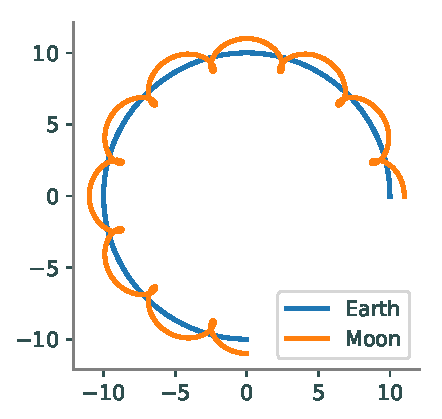
\includegraphics[width=.65\textwidth]{figures/SolarSystem.pdf}
\end{figure}

\label{prob:solar-system-trajectories}
 % Time Matrix-Vector and Matrix-Matrix Multiplication.
Let $A$ be an $m \times n$ matrix with entries $a_{ij}$, $\x$ be an $n \times 1$ vector with entries $x_k$, and $B$ be an $n \times p$ matrix with entries $b_{ij}$.
%
% \begin{align*}
% A = \left[\begin{array}{cccc}
% a_{11} & a_{12} & \cdots & a_{1n} \\
% a_{21} & a_{22} & \cdots & a_{2n} \\
% \vdots & \vdots & \ddots & \vdots \\
% a_{m1} & a_{m2} & \cdots & a_{mn}
% \end{array}\right]
% &&
% \x = \left[\begin{array}{c}
% x_1 \\ x_2 \\ \vdots \\ x_n
% \end{array}\right]
% &&
% B = \left[\begin{array}{cccc}
% b_{11} & b_{12} & \cdots & b_{1p} \\
% b_{21} & b_{22} & \cdots & b_{2p} \\
% \vdots & \vdots & \ddots & \vdots \\
% b_{n1} & b_{n2} & \cdots & b_{np}
% \end{array}\right]
% \end{align*}
%
The matrix-vector product $A\x = \y$ is a new $m \times 1$ vector and the matrix-matrix product $AB = C$ is a new $m \times p$ matrix.
The entries $y_i$ of $\y$ and $c_{ij}$ of $C$ are determined by the following formulas:
%
\begin{align*}
y_i = \sum_{k=1}^n a_{ik}x_k%,\qquad i = 1,\ 2,\ \ldots,\ m.
&&
c_{ij} = \sum_{k=1}^n a_{ik}b_{kj}%,\quad i = 1,\, 2,\, \ldots,\ m, \quad j = 1,\, 2\, \ldots,\ l.
\end{align*}

These formulas are implemented below \textbf{without} using NumPy arrays or operations.

\begin{lstlisting}
def matrix_vector_product(A, x):    # Equivalent to np.dot(A,x).tolist()
    """Compute the matrix-vector product Ax as a list."""
    m, n = len(A), len(x)
    return [sum([A[i][k] * x[k] for k in range(n)]) for i in range(m)]

def matrix_matrix_product(A, B):    # Equivalent to np.dot(A,B).tolist()
    """Compute the matrix-matrix product AB as a list of lists."""
    m, n, p = len(A), len(B), len(B[0])
    return [[sum([A[i][k] * B[k][j] for k in range(n)])
                                    for j in range(p) ]
                                    for i in range(m) ]
\end{lstlisting}

Time each of these functions with increasingly large inputs.
Generate the inputs $A$, $\x$, and $B$ with \li{random_matrix()} and \li{random_vector()} (so each input will be $n \times n$ or $n \times 1$).
Only time the multiplication functions, not the generating functions.

Report your findings in a single figure with two subplots: one with matrix-vector times, and one with matrix-matrix times.
Choose a domain for $n$ so that your figure accurately describes the growth, but avoid values of $n$ that lead to execution times of more than 1 minute.
Your figure should resemble the following plots.

\begin{figure}[H] % Generated with prob1_solution() in plots.py.
\captionsetup[subfigure]{justification=centering}
\centering
\begin{subfigure}{.5\textwidth}
    \centering
    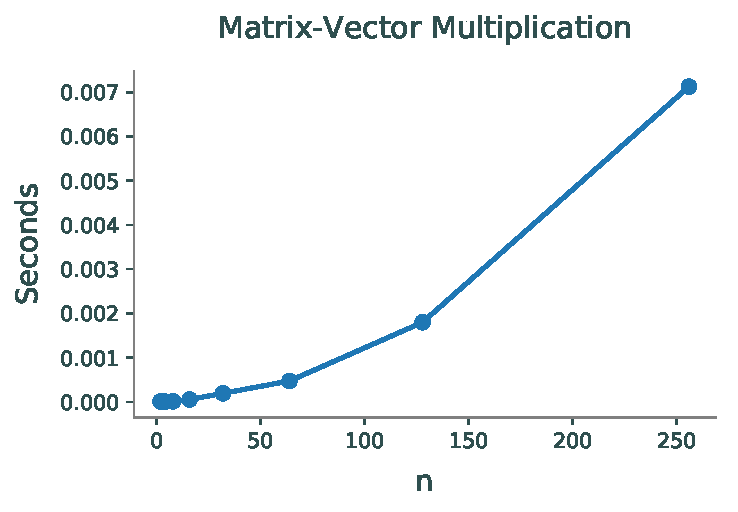
\includegraphics[width=\linewidth]{figures/matrixVectorMultiplication.pdf}
\end{subfigure}%
\begin{subfigure}{.482\textwidth}
    \centering
    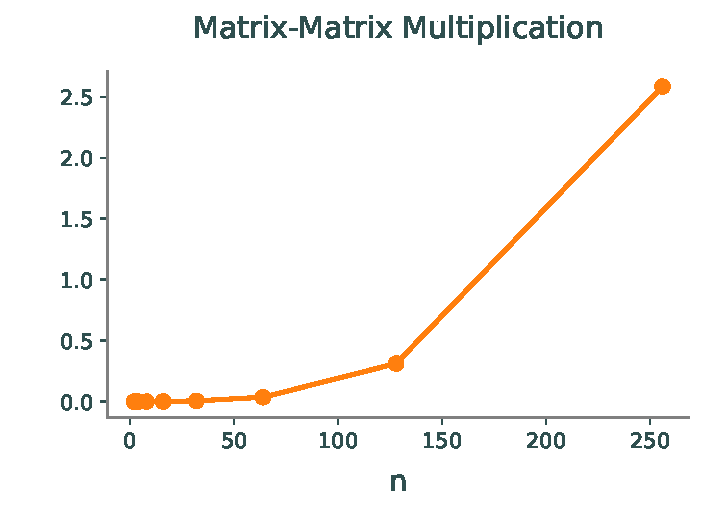
\includegraphics[width=\linewidth]{figures/matrixMatrixMultiplication.pdf}
\end{subfigure}
\end{figure}

\label{prob:matrix-multiplication-timing}
 % Why NumPy ROCKS.
NumPy is built specifically for fast numerical computations.
Repeat the experiment of Problem \ref{prob:matrix-multiplication-timing}, timing the following operations:
%
\begin{itemize}
\item matrix-vector multiplication with \li{matrix_vector_product()}.
\item matrix-matrix multiplication with \li{matrix_matrix_product()}.
\item matrix-vector multiplication with \li{np.dot()} or \li{@}.
\item matrix-matrix multiplication with \li{np.dot()} or \li{@}.
\end{itemize}

Create a single figure with two subplots: one with all four sets of execution times on a regular linear scale, and one with all four sets of execution times on a log-log scale.
Compare your results to Figure \ref{fig:loglogdemo}.
\label{prob:numpy-is-awesome}
